\subsection{Priklausomybių versijų pasirinkimas Go sistemoje}

Nuo pat „go get“ pristatymo, viena didžiausių šios komandos problemų buvo
nežinojimas apie valdomų paketų versijas.
Senoji „go get“ komanda turėjo du priklausomybių versijų pasirinkimo algoritmus.
Pirmasis, Go numatytasis algoritmas, „go get B“ metu atsiųsdavo naujausią paketo B versiją
bei naujausias B priklausomybes, kurių nebuvo turima lokaliai. Antrasis algoritmas įvykdžius „go get -u B“
atsiųsdavo naujausią B, bei visas naujausias jos tranzityvių priklausomybių versijas \textsuperscript{[COX18d]}.

Abu šie algoritmai netenkino vartotojų bei kėlė daug klaidų. Naudojant pirmąjį algoritmą,
kilo grėsmė, jog lokaliai turimos priklausomybės bus per senos ir neveiks su naujai atsiųstomis
priklausomybėmis. Antrasis algoritmas taip pat nebuvo visiškai saugus, nes buvo galimybė,
jog naujausios priklausomybių versijos nebus tarpusavyje sutapatinamos (ang. compatible) \textsuperscript{[COX18e]}.

%\begin{figure}[H]
%    \centering
%    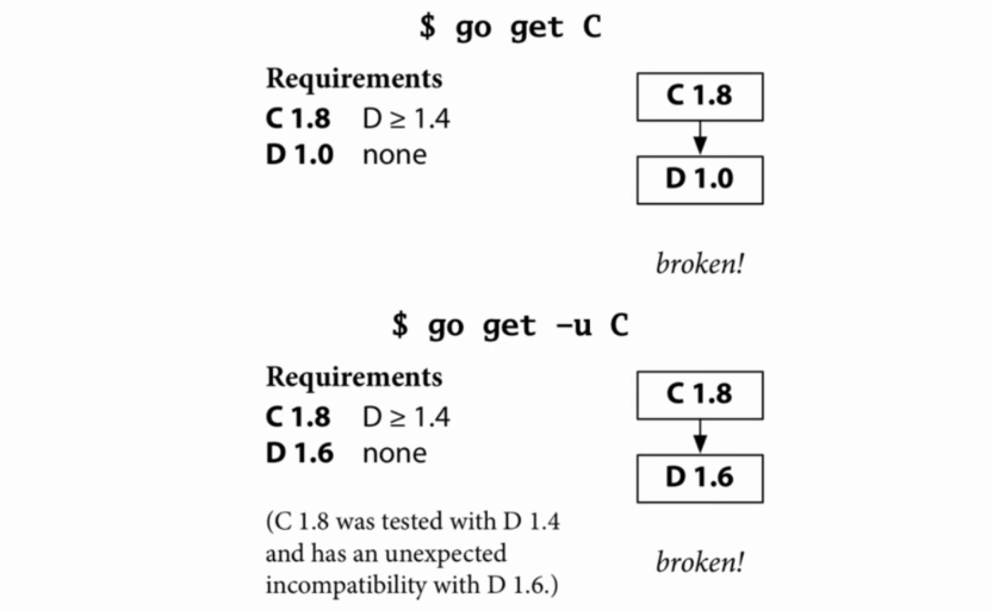
\includegraphics[width=\textwidth]{old_go_get}
%    \caption{Problemos „go get“ komandoje \textsuperscript{[COX18e]}}
%\end{figure}

Suprasdami „go get“ priklausomybių versijų pasirinkimo algoritmų keliamas problemas,
Go inžinieriai į pasiūlymą dėl version-aware Go komandos įtraukė ir naują algoritmą priklausomybių
versijų pasirinkimui. Šis algoritmas vadinasi „minimal version selection“ ir siūlo lyg šiol mažai naudotą
priklausomybių versijų pasirinkimo mechanizmą - pasirinkti seniausią leidžiamą paketo versiją.
Dauguma šiuolaikinių priklausomybių valdymo sistemų, tokių kaip dep ar cargo, naudoja priešingą algoritmą -
renkasi naujausią leidžiamą priklausomybės versiją \textsuperscript{[COX18a, COX18f]}.

Russ Cox, vienas pagrindinių Go kūrėjų, teigia, cargo bei dep naudojamas algoritmas yra klaidingas
dėl dviejų priežasčių. Pirmoji priežastis yra tai, jog naujausia leidžiama versija gali nuolat kisti
bei būti nestabili, antroji - klaidos atveju vartotojui reikia skirti papildomo
laiko uždrausti naudoti specifinių versijų priklausomybes \textsuperscript{[COX18a]}.

%\begin{figure}[H]
%    \centering
%    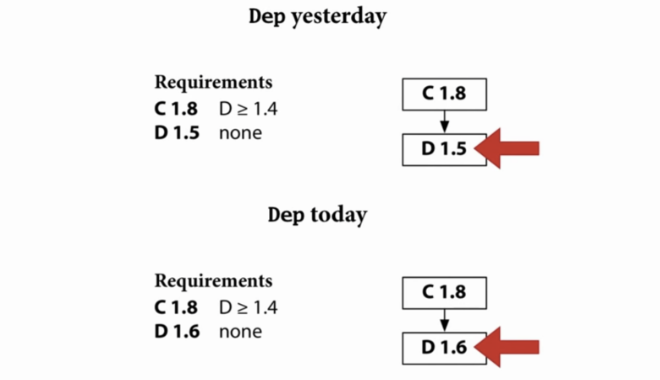
\includegraphics[width=\textwidth]{dep_working}
%    \caption{Naujausios leidžiamos versijos algoritmas dep sistemoje \textsuperscript{[COX18e]}}
%\end{figure}

Go inžinierių pasirinktas „minimal version selection“ algoritmas turi kelis pranašumus.
Šis algoritmas užtikrina, jog visada su ta pačia „go get“ komanda bus gaunamos tų pačių versijų priklausomybes.
Garantija, jog projekto priklausomybės nesikeis, leidžia užtikrinti, jog programos surinkimo rezultatas visada bus toks pats,
tiek programų sistemos kūrimo metu, tiek sistemos produkcinėje aplinkoje \textsuperscript{[COX18a]}. „Minimal version selection“ taip pat
leidžia apsisaugoti nuo naujausiose paketų versijose galinčių būti klaidų - jei paketo A naujausiose versijoje yra klaida,
tiek A paketo autorius, tiek kitų paketų, naudojančių A, autoriai turi laiko ištaisyti klaidą bei
uždrausti naudoti šią trikį turinčią versiją \textsuperscript{[COX18e]}.

%\begin{figure}[H]
%    \centering
%    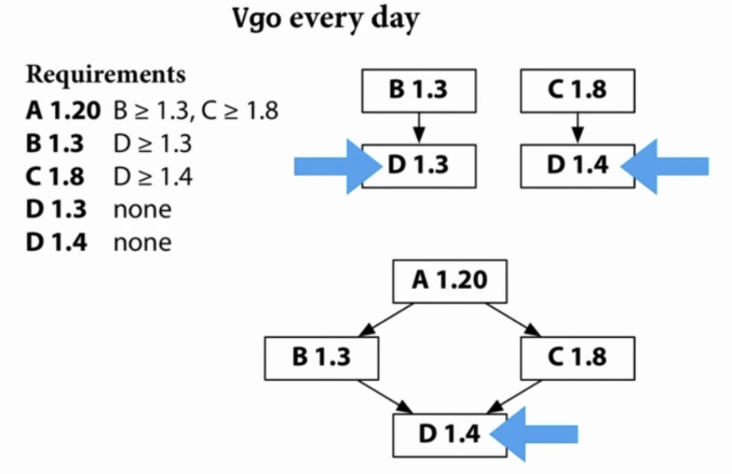
\includegraphics[width=\textwidth]{vgo_min_version}
%    \caption{„Minimal version selection“ \textsuperscript{[COX18e]}}
%\end{figure}
